\documentclass[resume.tex]{subfiles}


\begin{document}
\section{Codage de canal}
$$(n,k,d)_q$$
Lorsque la base est $q=2$ on ne l'affiche pas
\begin{center}
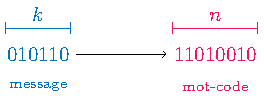
\includegraphics[scale=1,page=1]{drwg_1.pdf}
\end{center}
\begin{center}
\begin{tabular}{c|l}
$k$ & Nombre de bits à transmettre (information)\\
$n$ & Nombre de bits transmis $n\geq k$\\
$d$ & Distance de Hamming
\end{tabular}
\end{center}
Information (bits à transmettre)
$$x=\begin{pmatrix}
x_{k-1} &
x_{k-2} &
\cdots &
x_1 &
x_0
\end{pmatrix}\in \mathbb{R}^{1\times k}$$
Matrice systématique (identité à gauche).
$$G_S=\begin{pmatrix}
\textcolor{RoyalBlue}{I_k} & \textcolor{OrangeRed}{P}
\end{pmatrix}=
\left(\begin{array}{cccc|cccc}
\textcolor{RoyalBlue}{1} & \textcolor{RoyalBlue}{0} & \cdots & \textcolor{RoyalBlue}{0} & \textcolor{OrangeRed}{x} & \cdots & \textcolor{OrangeRed}{x}\\
\textcolor{RoyalBlue}{0} & \textcolor{RoyalBlue}{1} & \cdots & \textcolor{RoyalBlue}{0} & \textcolor{OrangeRed}{x} & \cdots & \textcolor{OrangeRed}{x}\\
\vdots & \vdots & \ddots & \vdots & \vdots & \ddots & \vdots\\
\textcolor{RoyalBlue}{0} & \textcolor{RoyalBlue}{0} & \cdots & \textcolor{RoyalBlue}{1} & \textcolor{OrangeRed}{x} & \cdots & \textcolor{OrangeRed}{x}
\end{array}\right)\in\mathbb{R}^{k\times n}$$
$$H_s=\begin{pmatrix}
\textcolor{OrangeRed}{P^{T}} & \textcolor{RoyalBlue}{I_{n-k}}
\end{pmatrix}\in\mathbb{R}^{n-k\times n}$$
Capacité de détection d'erreurs : $d_{min}-1$\\
Capacité de correction d'erreurs : $\left\lfloor\frac{d_{min}-1}{2}\right\rfloor$


\subsection{Propriétés}
$$G_SH_S^T=0$$
\subsection{Codes polynomiaux}
\begin{enumerate}
\item Souvent linéaires (+ parfois cycliques)
\item Générateur rarement systématique (on peut utiliser un encodage systématique si le générateur ne l'est pas)
\end{enumerate}
\subsection{Codes linéaires}
La somme de deux codes valides donne un nouveau code valide
\subsection{Codes cycliques}
Un décalage vers la gauche $\textcolor{OrangeRed}{0}011\longrightarrow 011\textcolor{OrangeRed}{0}$ ou vers la droite $001\textcolor{OrangeRed}{1}\longrightarrow \textcolor{OrangeRed}{1}001$ donne un autre code valide.\\
Un décalage d'un mot-code de longueur $n$ dans $\mathbb{R}_n[X]$ est similaire à une multiplication par $X$
\subsubsection{Générateur}
Un générateur permet, par des décalages cycliques et des sommes d'obtenir tous les mots-code.\\
Si le générateur divise $(1+X^n)$ alors le code est cyclique
\subsubsection{Encodage}
On veut encoder un message $x$ et obtenir le mot-code $y$
\paragraph{Encodage systématique} :
$$x\xrightarrow{\text{encodage}} xX^{n-k}+\text{reste}\left(\frac{xX^{n-k}}{g(x)}\right)=y$$
Les bits du message se retrouvent au début du mot-code
\paragraph{Encodage "standard"} :
$$x\xrightarrow{\text{encodage}} xg(x)=y$$
\subsubsection{Vérification}
On va simplement chercher à savoir si le message est correct ou non.\\
Vérification systématique (on vérifie simplement que le message soit égal au reste, comme pour l'encodage)
$$y[0:k] == \text{reste}\left(\frac{y[0:k]X^{n-k}}{g(x)}\right)$$
Vérification "standard"
$$s(x)=e(x)=\frac{y}{g(x)}\qquad s(x)=0\longrightarrow\text{ ok}$$
\subsubsection{Correction d'erreurs}
On va utiliser une matrice de contrôle (typiquement pour les codes BCH) qui va indiquer la position de(s) erreur(s)
\subsubsection{Décodage}
Dans le cas où le message est correct, on va effectuer le décodage.\\
Décodage systématique (on récupère simplement les bits dans le message tels-quels):
$$\hat{x}=y[0:k]$$
Décodage "standard" :
$$\hat{x}=\frac{y}{g(x)}$$
\subsection{Générateur $\leftrightarrow$ matrice}
On peut créer la matrice en effectuant des décalages cycliques du générateur $g(x)$
$$\underset{k\times n}{\begin{pmatrix}
g_0 & g_1 & \cdots & g_{n-k} & 0 & 0\\
0 & g_0 & g_1 & \cdots & g_{n-k} & 0\\
0 & 0 & g_0 & g_1 & \cdots & g_{n-k}\\
\end{pmatrix}}$$
Avec le nombre de lignes correspondant à la longueur du message. Cette matrice n'est pas systématique. Il faut la manipuler si on veut obtenir la version systématique.\\
On effectue ensuite des combinaisons linéaires sur les lignes pour obtenir la matrice systématique.
\subsection{Codage convolutionnel}

\end{document}